\section{Introduction}

\subsection{Preface}
\texttt{PyCorrFit} emerged from my work in the Schwille Lab\footnote{\url{http://www.biochem.mpg.de/en/rd/schwille/}} at the Biotechnology Center of the TU Dresden in 2011/2012. The program source code is available at GitHub\footnote{\url{https://github.com/paulmueller/PyCorrFit}}. Please do not hesitate to sign up and add a feature request. If you you found a bug, please let me know via GitHub.\\

\noindent \texttt{PyCorrFit} was written to simplify the work with experimentally obtained correlation curves. These can be processed independently (operating system, location, time). PyCorrFit supports commonly used file formats and enables users to allocate and organize their data in a simple way.\\

\noindent PyCorrFit is free software: you can redistribute it and/or modify it
under the terms of the GNU General Public License as published 
by the Free Software Foundation, either version 2 of the License, 
or (at your option) any later version\footnote{\url{http://www.gnu.org/licenses/gpl.html}}.

\subsubsection*{What PyCorrFit can do}
\begin{itemize}
\item Load correlation curves from numerous correlators
\item Process these curves (e.g. background correction, s. Tools section \ref{sec:tools} )
\item Fit a model function (many included) to an experimental curve
\item Import user defined models for fitting
\item Many batch processing features
\item Save/load entire PyCorrFit sessions
\end{itemize}

\subsubsection*{What PyCorrFit is not}
\begin{itemize}
\item A multiple-$\tau$ correlator
\item A software to operate hardware correlators
\end{itemize}

\subsection{System prerequisites}
\subsubsection{Hardware}
This documentation addresses the processing of correlation curves with PyCorrFit. {PyCorrFit} was successfully used with the following setups:
\begin{itemize}
\item[1.]
     APD: Photon Counting Device from PerkinElmer Optoelectronics, Model: 	 \texttt{SPCM-CD3017}\\
     Correlator: Flex02-01D/C from correlator.com with the shipped software 	
	    		 \texttt{flex02-1dc.exe}.
\item[2.]
    APD: Photon Counting Device from PerkinElmer Optoelectronics\\
    Correlator: ALV-6000
\item[3.] LSM Confocor2 or Confocor3 setups from Zeiss, Germany.
\end{itemize}

\subsubsection{Software}
\label{cha:soft}
The latest version of PyCorrFit can be obtained from the internet at \url{http://pycorrfit.craban.de}.
\begin{itemize}
\item \textbf{MacOSx}.
Binary files for MacOSx $>$10.6.8 are available from the download page but have not yet been fully tested for stability.
\item \textbf{Windows}.
For Windows XP or Windows 7, stand-alone binary executables are available from the download page. 
\item \textbf{Linux}.
There are executable binaries for widely used distributions (e.g. Ubuntu).
\item \textbf{Sources}
The program was written in Python, keeping the concept of cross-platform programming in mind. To run PyCorrFit on any other operating system, the installation of Python v.2.7 is required. To obtain the latest source, visit PyCorrFit at GitHub (\url{https://github.com/paulmueller/PyCorrFit}). PyCorrFit depends on the following python modules:\\
\texttt{\\
python-matplotlib ($\geq$ 1.0.1) \\
python-numpy ($\geq$ 1.5.1) \\
python-scipy ($\geq$ 0.8.0) \\
python-sympy ($\geq$ 0.7.2) \\
python-yaml \\
python-wxtools \\
python-wxgtk2.8-dbg \\
}
\\
For older versions of Ubuntu, some of the above package versions are not listed in the package repository. To enable the use of PyCorrFit on those systems, the following tasks have to be performed:
\begin{itemize}
\item[ ] \textbf{matplotlib}. The tukss-ppa includes version 1.0.1. After adding the repository (\texttt{apt-add-repository ppa:tukss/ppa}), matplotlib can be installed as usual.
\item[ ] \textbf{numpy}. The package from a later version of Ubuntu can be installed: \url{https://launchpad.net/ubuntu/+source/python-numpy/}
\item[ ] \textbf{scipy}. The package from a later version of Ubuntu can be installed: \url{https://launchpad.net/ubuntu/+source/python-scipy/}
\item[ ] \textbf{sympy}. To enable importing external model functions, sympy is required. It is available from \url{http://code.google.com/p/sympy/downloads/list}. Unpacking the archive and executing \texttt{python setup.py install} within the unpacked directory will install sympy.
\end{itemize}
\end{itemize}
Alternatively \texttt{python-pip} (\url{http://pypi.python.org/pypi/pip}) can be used to install up-to-date python modules.

\noindent \textbf{\LaTeX}.
PyCorrFit can save correlation curves as images using matplotlib. It is also possible to utilize Latex to generate these plots. On Windows, installing MiKTeX  with ``automatic package download'' will enable this feature. On MacOSx, the MacTeX distribution can be used. On other systems, the packages LaTeX, dvipng, Ghostscript and the scientific latex packages \texttt{texlive-science} and \texttt{texlive-math-extra} need to be installed.

\subsection{Running PyCorrFit}
\label{sec:run}
\paragraph*{Windows}
Download the executable file and double-click on the \texttt{PyCorrFit.exe} icon.
\paragraph*{Linux/Ubuntu}
Make sure the binary has the executable bit set, then simply double-click on the binary  \texttt{PyCorrFit}.
\paragraph*{Mac OSx}
When downloading the archive \texttt{PyCorrFit.zip}, the binary should be extracted automatically (if not, extract the archive) and you can double-click it to run PyCorrFit.
\paragraph*{from source}
Invoke \texttt{python PyCorrFit.py} from the command line.


\section{Working with PyCorrFit}

\subsection{Workflow}
\label{cha_graphint}
\label{sec:PyCorrFitUserInterface}

The following chapter introduces the general idea of how to start and accomplish a fitting project. FCS experiments produce different sets of experimental correlation functions which must be interpreted with appropriate physical models. Each correlation function refers to a single contiguous signal trace or ``run''. In \textit{PyCorrFit}, the user must assign a mathematical model function to each correlation function during the loading procedure. The assignment is irreversible in the sense that within an existing \textit{PyCorrFit} session it cannot be changed. This feature assures the stability of the batch processing routine for automated fitting of large data sets. Nevertheless, the fit of different models to the same data can be explored by loading the data twice or simply by creating two different sessions.

Let's briefly discuss a typical example: To determine the diffusion coefficient of a fluorescently labeled protein in free solution, one has to deal with two sets of autocorrelation data: measurements of a diffusion standard (e.g. free dye for which a diffusion coefficient has been published) to calibrate the detection volume and measurements of the protein sample. The protein sample may contain small amounts of slowly diffusing aggregates. While the calibration measurements can be fitted with a one-component diffusion model (T-3D), the protein sample displays two mobility states, monomers and aggregates, which are taken into account by a two-component diffusion model (T-3D-3D). With \textit{PyCorrFit} such a situation can be treated in three ways, having different pros and cons: 


\begin{enumerate}
\item Create separate sessions for each type of sample and assign different model functions.
\item Assign a one-component model to the dye measurements and a two-component model to the protein measurements when loading consecutively into the same session.
\item Assign a two-component model for all data and, when appropriate, manually inactivate one component by fixing its contribution to 0\%.
\end{enumerate}


The first approach is straightforward, however, it requires homogeneous diffusion behavior for each data set. The second strategy has the advantage that the dye and the protein curves, as well as the obtained parameters can be visually compared during the fitting analysis within the same session. In this case, batch fitting is still possible because it discriminates data sets assigned to different models. In the third case, simultaneous batch fitting is also possible. However, for each dye measurement one has to eliminate the second, slow diffusion species manually, which might be laborious. Inactivating components by fixing parameters is nevertheless a common way to evaluate heterogeneous data sets, for example, a protein sample for which only a subgroup of curves requires a second diffusion component due to occasional appearance of aggregates. Such situations are frequently encountered in intracellular measurements. In conclusion, all three strategies or combinations thereof may be suitable. In any case, the user must decide on model functions beforehand, therefore it is advisable to group the data accordingly.

The fitting itself is usually explored with a representative data set. Here, the user has to decide on starting parameters, the range in which they should be varied, corrections like background, and other fitting options. Once the fit looks good, the chosen settings can be transferred at once to all other pages assigned to the same model using the \textit{Batch control} tool (\hyref{Section}{sec:tm.bc}). After flipping through the data for visual inspection one may check the parameters across all pages in the \textit{Statistics view} tool and re-visit outliers (\hyref{Section}{sec:tm.sv}). From there, the numerical fit values and example correlation functions can be exported.

\subsection{The \textit{main window}}

%\hyref{Figure}{fig:PyCorrFitMain} shows the main window of PyCorrFit. It contains a menu bar to access all tools, a notebook with tabs, each tab representing a single curve, and a page - the content of the currently selected tab. 


Together with a system's terminal of the platform on which PyCorrFit was installed (Windows, Linux, MacOS), the \textit{main window} opens when starting the program as described in \hyref{section}{sec:run}. The window title bar contains the version of \textit{PyCorrFit} and, if a session was re-opened or saved, the name of the fitting session. A menu bar provides access to many supporting tools and additional information as thoroughly described in \hyref{Chapter}{sec:mb}. 

There are three gateways for experimental data into a pre-existing or a new \textit{PyCorrFit} session (\textit{File / Load data}, \textit{File / Open session}, and \textit{Current page / Import data}). When a session has been opened or correlation data have been loaded, each correlation curve is displayed on a separate page of a notebook. For quick identification of the active data set, a tab specifies the page number, the correlated channels (AC/CC), and the run number in case there are multiple runs in one experimental data file. When clicking a little triangle to the far-right, one can use a drop-down list of all page titles to directly access a particular data set. Alternatively, the pages can be toggled by tapping the curser keys (left/right). There can be only one activated page for which the tab appears highlighted.

\begin{figure}[h]
\centering
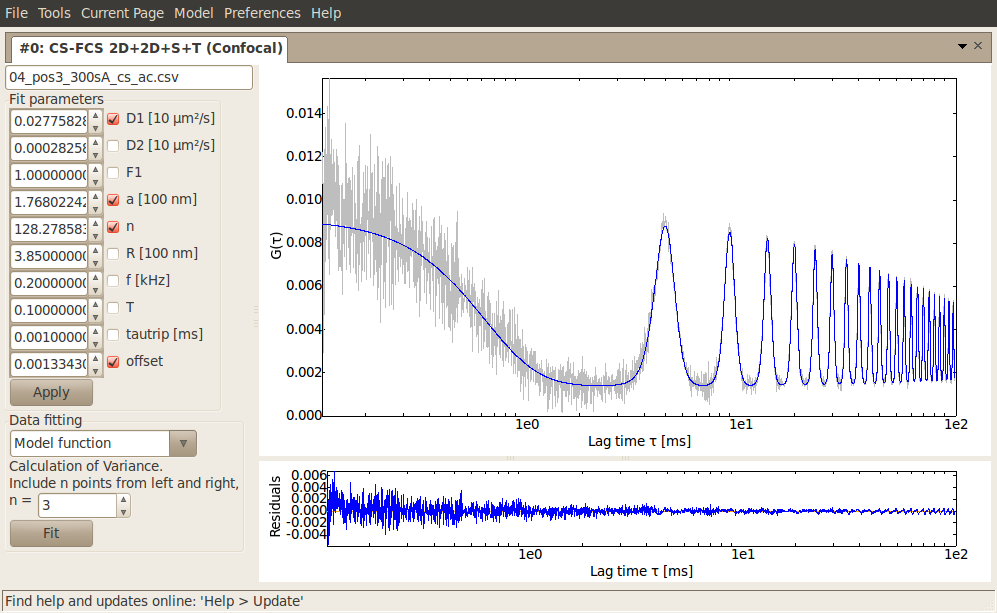
\includegraphics[width=\linewidth]{PyCorrFit_Screenshot_Main.png}
 \mycaption{user interface of PyCorrFit}{A circular scanning FCS (CS-FCS) curve of DiO on a supported lipid bilayer (glass substrate) is shown. The measurement yields a diffusion coefficient of \SI{0.28}{\mu m^2s^{-1}} ($F1=1$, so only one component is fitted). Note that a 2D diffusion model is used and not a 3D model (as shown in \hyref{figure}{fig:extxt}). \label{fig:PyCorrFitMain}}
\end{figure}

The page containing a correlation function is divided in two halves. At the left hand side the page\textit{ }shows a pile of boxes containing values or fitting options associated to the current model and data set: 



\begin{itemize}
\item \textit{Data set}, a unique identifier for each correlation curve which is automatically assembled from different fields during the loading procedure (\hyref{Section}{sec:fm.ld}). This window can also be manually edited, thereby allowing to re-name or flag certain data during the fitting analysis. 
\item \textit{Model parameters} displays the values which determine the current shape of the assigned model function. Initially, starting values are loaded as they were defined in the model description (\hyref{Section}{sec:fm.im}). Little buttons allow a stepwise increase or decrease in units of 1/10\textsuperscript{th}. It is also possible to directly enter some numbers. A checkbox is used to set the parameter status to ``varied'' (checked) or ``fixed'' (unchecked) during the fitting. At the end, when saving the session, the current set of values together with their indicated names are stored in the *.yaml file (\hyref{Section}{sec:fm.ss}). 
\item \textit{Amplitude corrections} applies additional rescaling to amplitude related parameters like the number of particles $n$ or fractions thereof associated with different correlation times ($n_1$, $n_2$, etc.). Experimental values of non-correlated background intensity can be manually entered for each channel. In addition, the correlation curves can be normalized, to facilitate a visual comparison of their time dependence.
\item \textit{Fitting options} offers weighted fitting. The underlying idea is that data points with higher accuracy should also have a higher impact on model parameters. To derive weights, \textit{PyCorrFit} calculates the variance of the difference between the actual data and a smooth, empiric representation of the curve for a certain neighborhood. The number of neighboring data points at each side ($j > 0$) can be set. For such a smooth representation a 5-knot spline function or the model function with the current parameter set can be used. The latter should improve when repeatedly fitting.
\end{itemize}
At the right hand side are two graphics windows. The dimensionless correlation functions $G(\tau)$ are plotted against the lag time ($\tau$) in logarithmic scale. Below, a second window shows the residuals, the actual numerical difference between the correlation data and the model function. Fitting with appropriate models will scatter the residuals symmetrically around zero ($x$-axis). When weighted fitting was performed, the weighted residuals are shown. A good fit will not leave residuals systematically above or below the $x$-axis at any time scale.

The main window can be rescaled as a whole to improve data representation. In addition, to zoom in, one can drag a rectangle within the plot area; a double click then restores the initial scale. Experimental data points are linked by grey lines, the state of the model function is shown in blue. When a weighted fit was applied, the variance of the fit is calculated for each data point and displayed in cyan.

\section{The menu bar}
\label{sec:mb}

PyCorrFit is organized in panels which group certain functions. The menu organizes data management (File), data analysis (Tools), display of correlation functions (Current Page), numerical examples (Model), software settings (Preferences), and software metadata (Help). The documentation refers to the version 0.8.1.

\subsection{File menu}
\label{sec:fm}
The File menu organizes the import of theoretical models, experimental correlation data, and opening and saving of entire \textit{PyCorrFit} fitting sessions. However, the numerical fit results are exported from the \textit{Statistics view} panel which can be found under \textit{Tools} (\hyref{Section}{sec:tm.sv}).

\subsubsection{File / Import model}
\label{sec:fm.im}
Correlation data must be fitted to models describing the underlying physical processes which give rise to a particular time dependence and magnitude of the recorded signal fluctuations. Models are mathematical expressions containing parameters with physical meaning, like the molecular brightness or the dwell time through an illuminated volume etc. While a number of standard functions are built-in, the user can define new expressions. Some examples can be found at GitHub in the \textit{PyCorrFit} repository, e.g. circular scanning FCS [REF] or a combination of diffusion and directed flow [REF].

Model functions are imported as text files (*.txt) using certain syntax:

\begin{itemize}
\item \textbf{Encoding}: PyCorrFit can interpret the standard Unicode character set (UTF-8).
\item \textbf{Comments}: Lines starting with a hash (\#), empty lines, or lines containing only white space characters are ignored. The only exception is the first line starting with a hash followed by a white space and a short name of the model. This line is evaluated to complement the list of models in the dialogue\textit{ Choose }\textit{model}, when loading the data.
\item \textbf{Units}: PyCorrFit works with internal units for:

\begin{itemize}
\item Time: \SI{1}{ms}
\item Distance: \SI{100}{nm}
\item Diffusion coefficient: \SI{10}{\mu m^2s^{-1}} 
\item Inverse time: \SI{1000}{s^{-1}} 
\item Inverse area: \SI{100}{\mu m^{-2}} 
\item Inverse volume: \SI{1000}{\mu m^{-3}} 
\end{itemize}
\item \textbf{Parameters:} To define a new model function new parameters can be introduced. Parameters are defined by a sequence of strings separated by white spaces containing name, the dimension in angular brackets, the equal sign, and a starting value which appears in the main window for fitting. For example: D [50 µm\textsuperscript{2}s\textsuperscript{{}-1}] = 50.00. It is important to note that when the dimensions differ from the internal units (10 µm\textsuperscript{2}s\textsuperscript{{}-1}), the expression must contain some adjusting factor; here a factor of 5. Thus, user defined dimensions are only for display and cannot be processed numerically. The parameter names contain only alphabetic (not numerical) characters. ‘G’ and ‘g’, as well as the numbers ‘e’ and ‘pi’ are already mapped and cannot be used freely.
\item \textbf{Placeholder:} When defining composite mathematical expressions for correlation functions one can use placeholders. Placeholders start with a lowercase ‘g’. For example, the standard, Gaussian 3D diffusion in free solution may be written as

\begin{itemize}
\item \texttt{gTrp = 1+ T/(1-T)*exp(-tau/tautrip)}
\item \texttt{gTwoD = 1/(1+tau/taudiff)}
\item \texttt{gThrD = 1/sqrt(1+tau/(taudiff*S**2))}
\end{itemize}
\end{itemize}
The individual parts are then combined in the last line of the *.txt file, where the correlation function is defined starting with uppercase ’G’:

\begin{equation}
\texttt{G = 1/n * gTrp * gTwoD * gThrD} \notag
\end{equation}
For reference of mathematical operators check for example \href{http://www.tutorialspoint.com/python/python_basic_operators.htm}{www.tutorialspoint.com / python / python\_basic\_operators.htm}. To illustrate a more complex example see the model function for circular scanning FCS in \hyref{figure}{fig:extxt}. 


\begin{figure}
% for case sensitiver Verbatim, we need the package fancyvrb
\begin{Verbatim}[frame = single]

# CS-FCS 3D+S+T (Confocal)

# Circular Scanning FCS model function. 3D diffusion + Triplet.

## Definition of parameters:
# First, the parameters and their starting values for the model function
# need to be defined. If the parameter has a unit of measurement, then it 
# may be added separated by a white space before the "=" sign. The starting
# value should be a floating point number. Floating point abbreviations 
# like "1e-3" instead of "0.001" may be used.

# Diffusion coefficient
D [10 µm²/s] = 200.0
# Structural parameter
w = 5.0
# Waist of the lateral detection area
a [100 nm] = 1.0
# Particle number
n = 5.0
# Scan radius
R [100 nm] = 5.0
# Frequency
f [kHz] = 20.0
# Triplet fraction
T = 0.1
# Triplet time
tautrip [ms] = 0.001

# The user may wish to substitute certain parts of the correlation function
# with other values to keep the formula simple. This can be done by using the
# prefix "g". All common mathematical functions, such as "sqrt()" or "exp()"
# may be used. For convenience, "pi" and "e" are available as well.

gTrip = 1. + T/(1-T)*exp(-tau/tautrip)
gScan = exp(-(R*sin(pi*f*tau))**2/(a**2+D*tau))
gTwoD = 1./(1.+D*tau/a**2)
gOneD = 1./sqrt(1.+D*tau/(w*a)**2)
gThrD = gTwoD * gOneD

# The final line with the correlation function should start with a "G"
# before the "=" sign.

G = 1./n * gThrD * gScan * gTrip

\end{Verbatim}
\mycaption{user defined model function for PyCorrFit}{The working example shows a model function for circular scanning FCS.\label{fig:extxt}}
\end{figure}


\subsubsection{File / Load data}
\label{sec:fm.ld}
\textit{Load data }is the first way to import multiple correlation data sets into a \textit{PyCorrFit} session. The supported file formats can be found in a drop-down list of supported file endings in the pop-up dialog \textit{Open data files}:


\begin{enumerate}
\item All supported files \ \ \ \ \ \ [default]
\item Confocor3 (*.fcs)\ \ \ \ \ \ [AIM 4.2, ZEN 2010, Zeiss, Germany]
\item Correlator ALV6000 (*.ASC)\ \ [ALV Laser GmbH, Langen, Germany]
\item Correlator.com (*.SIN)\ \ \ \ [www.correlator.com, USA]
\item Matlab ‘Ries (*.mat)\ \ \ \ \ \ [EMBL Heidelberg, Germany]
\item PyCorrFit (*.csv)\ \ \ \ \ \ [Paul Müller, TU Dresden, Germany]
\item Zip files (*.zip)\ \ \ \ \ \ [Paul Müller, TU Dresden, Germany]
\end{enumerate}
While (1)-(4) are file formats associated with commercial hardware, (5) refers to a MATLAB based FCS evaluation software developed by Jonas Ries in the Schwille lab at TU Dresden, (6) is the txt-file containing comma-separated values (csv) generated with PyCorrFit via the command \textit{Current Page / Save data}. Zip-files are automatically decompressed and can be imported when matching one of the above mentioned formats. In particular loading of zip files is a possibility to re-import correlation data from entire \textit{PyCorrFit} sessions. However, these data are treated as raw, which means that all fitting parameters and model assignments are lost.

When loading data, the user is prompted to assign fit models in the \textit{Choose }\textit{Models} dialogue window. There, curves are sorted according to channel (for example AC1, AC2, CC12, and CC21, as a typical outcome of a dual-color cross-correlation experiment). For each channel a fit model must be selected from the list (see Section 3.4 and Appendix xxx):

If a file format is not yet listed, the correlation data could be converted into a compatible text-file (*.csv) or bundles of *.csv files within a compressed archive *.zip. For reformatting the following points should be considered:


\begin{itemize}
\item \textbf{Encoding}: \textit{PyCorrFit} uses the standard Unicode character set (UTF-8). However, since no special characters are needed to save experimental data, other encodings may also work. New line characters are {\textbackslash}r{\textbackslash}n (Windows).
\item \textbf{Comments}: Lines starting with a hash (\#), empty lines, or lines containing only white space characters are ignored. Exceptions are the keywords listed below.
\item \textbf{Units}: PyCorrFit works with units/values for:

\begin{itemize}
\item Time: 1 ms
\item Intensity: 1 kHz
\item Amplitude offset: G(0) = 0 (not 1)
\end{itemize}
\item \textbf{Keywords: }\textit{PyCorrFit} reads the first two columns containing numerical values. The first table (non-hashed) is recognized as the correlation data containing the lag times in the first and the correlation data in the second column. (In case the *.csv file has been generated with \textit{PyCorrFit} up to three additional columns containing the fit function are ignored, see Section 3.1.6). The table ends, when the keyword \# BEGIN TRACE appears. Below this line the time and the signal values should be contained in the first two columns. If cross-correlation data have to be imported a second trace can be entered after the keyword \# BEGIN SECOND TRACE.
\item \textbf{Tags:} Channel information can be entered using defined syntax in a header. The keyword \# Type AC/CC Autocorrelation [uppercase?] assigns the tag ‘AC’ and \# Type AC/CC Cross-correlation assigns the tag ‘CC’ to the correlation curve. These strings are consistently displayed in the user interface of the respective data page in \textit{PyCorrFit}. If no data type is specified, autocorrelation is assumed. Tags may be specified with additional information like channel numbers, e.g. \# Type AC/CC Autocorrelation \_01. In this case the tag ‘AC\_01’ is generated. This feature is useful to keep track of the type of curve during the fitting and when post-processing the numerical fit results.
\end{itemize}

\subsubsection{File / Open session}
\label{sec:fm.os}
This command is the second way to import data into PyCorrFit. In contrast to \textit{Load data}, it opens an entire fitting project, which was previously saved with \textit{PyCorrFit}. Sessions are bundles of files named *.fcsfit-session.zip. Sessions contain, comments, model assigned correlation data, and the current state of parameters for each data page (Section 3.1.6).

\subsubsection{File / Comment session}
\label{sec:fm.cs}
This command opens a window to place text messages that can be used to annotate a fitting session.

\subsubsection{File / Clear session}
\label{sec:cls}
This command closes all pages while the PyCorrFit.exe keeps running. The user is prompted to save the session under the same or a different name. At this stage both options \textit{No} or \textit{Cancel} lead to clearance and a potential loss of recent modifications.

\subsubsection{File / Save session}
\label{sec:fm.ss}
In addition to display and fit individual curves, a strong feature of PyCorrFit is to save an entire fitting project as a single session. Sessions allow the user to revisit and explore different models, fitting strategies, and data sets. Importantly the work can be saved at any stage.

The number of files bundled in a session varies depending on the number of data sets (pages), the number of used models, and what was done during the fitting. A detailed description can be found in the Readme.txt file attached to each session. For example, the numerical correlation and intensity data are saved separately as *.csv text files. However, in contrast to the \textit{Save data (*.csv)} command of the \textit{Current Page} menu, there are no metadata in the header, just tables containing the numerical values. In sessions, the fitting parameters are stored separately in the human-readable data serialization format, *.yaml.

\subsubsection{File / Exit}
\label{sec:fm.e}
This command closes down \textit{PyCorrFit}. The user is prompted to save the session under the same or a different name. At this stage \textit{No} leads to the loss of recent changes, while \textit{Cancel} keeps \textit{PyCorrFit} running.

\subsection{Tools menu}
\label{sec:tm}
The \textit{Tools} menu provides access to a series of accessory panels which extent the capability of the main window. These accessory panels can stay open during the entire analysis. Open panels appear checked in the menu. Most operations can be executed across the entire data set with a single mouse click. 

\subsubsection{Tools / Data range}
\label{sec:tm.dr}
This panel limits the range of lag times which are displayed in the main window panel. At the same time it defines the range of points which are used for fitting. For example, this feature can be applied to remove dominant after-pulsing of the avalanche photo diodes (APDs) which may interfere with Triplet blinking at short lag times. The user has the options to \textit{Apply} the channel settings only to the current page or he can \textit{Apply to all pages}. In contrast to \textit{Batch control}, this operation ignores whether the data are assigned to different models. 

Power user, who frequently load and remove data sets, may take advantage of a checkbox to fix the channel selection for all newly loaded data sets.

\subsubsection{Tools / Overlay curves}
\label{sec:tm.oc}
This window displays the correlation data (not the fit curves) of all pages in a single plot. The curves can be discriminated by color. If only one curve is selected it appears in red. Curves with ambiguous shape can easily be identified, selected, and removed by clicking \textit{Apply}. A warning dialogue lists the pages which will be kept.

Data representation is synchronized with the page display in the \textit{Main window}. For example, narrowing the range of lag times by \textit{Data range }is immediately updated in the \textit{Overlay curves }tool. Likewise, their normalization of the amplitudes to unity.

The other way round, some tools directly respond to the selections made in the \textit{Overlay curves} tool: \textit{Global fitting}, \textit{Average curves}, and \textit{Statistics view} allow to perform operations on an arbitrary selection of pages which can be specified by page number. Instead of manually typing their numbers, the curves may be selected within the \textit{Overlay curves} tool. The respective input fields are immediately updated.

The tool is closed by the button \textit{Cancel}. All the listed data sets will be kept. However, the selections transferred to the \textit{Global fitting}, \textit{Average curves}, and \textit{Statistics view} tools are kept as well.

\subsubsection{Tools / Batch control}
\label{sec:tm.bc}
By default the current page is taken as a reference to perform automated fitting. A batch is defined as the ensemble of correlation data sets (pages) assigned to the same model function within a session. A session can therefore have several batches, even for the same data. 

For fitting it is crucial to carefully define the starting parameters, whether parameters should be fixed or varied, the range of values which make physically sense, and other options offered within the \textit{Main window}. By executing \textit{Apply to applicable pages}, these settings are transferred to all other pages assigned to the same fit model. Note that this includes the range of lag times (lag time channels) which may have been changed with the \textit{Data range }tool for individual pages.

The button \textit{Fit applicable pages} then performs several cycles of fitting [how many cycles?] on all pages of the same batch. Alternatively, the user can define an external source of parameters as a reference, i.e. the first page of some \textit{Other session} (*.fcsfit-session.zip). However, this assumes a consistent assignment of model functions.

\subsubsection{Tools / Global fitting}
\label{sec:tm.gf}
Global fitting is useful when experimental curves share the same values for certain physical parameters. For example, due to physical constraints in two-focus FCS both autocorrelation curves and the cross-correlation curves should adopt the same values for the diffusion time \textit{taudiff} and the number of particles \textit{n}. A global fit can be applied such that \textit{n} and \textit{taudiff} are identical for all data sets. All curves are added to a single array. In contrast to fixing the shared parameters across a batch, in \textit{Global fitting} Chi-square is minimized for all data sets simultaneously [please check!]. To perform \textit{Global fitting}, a subset of curves has to be selected by typing the numbers into the input field or by highlighting the pages via the \textit{Overlay} tool. 

\subsubsection{Tools / Average data}
\label{sec:tm.ad}
Often in FCS, the measurement time at a particular spot is divided in several runs. This approach is taken when occasional, global intensity changes are superimposed on the molecular fluctuations of interest. Then the user has to sort out the bad runs. After fitting, one may want to re-combine the data, to export a cleaned, average correlation function. This can be done with the tool \textit{Average data}, for which a subset of curves has to be selected by typing the numbers into the input field or by highlighting the pages via the \textit{Overlay curves} tool. 

For averaging, there are constraints:


\begin{enumerate}
\item Since the correlation curves are averaged point by point this requires the same number of lag time channels. Runs of different length cannot be averaged.
\item The tool can only average data sets which are exclusively autocorrelation or cross-correlation.
\item The user can check a box to enforce the program to ask for data sets with the same model as the current page. This may help to avoid mistakes when selecting pages.
\end{enumerate}
The averaged curve is shown on a separate page. The new \textit{Filename/title} receives the entry \textit{Average [numbers of pages]}. The assigned model is by default the same as for the individual pages. However, while averaging, the user can choose a different model from a drop-down list. 

\subsubsection{Tools / Trace view}
\label{sec:tm.tv}
FCS theory makes assumptions about the thermodynamic state of the system. Signal fluctuations can only be analyzed when the system is at equilibrium or at a sufficiently stable steady state. Global instabilities on the time scale of the measurement itself, e.g. photo-bleaching, have dramatic effect on the shape of the measured correlation curve. Therefore it is common practice to check the correlated intensity trace for each curve. Trace view simply displays the signal trace for each correlation function. The window stays open during the session and can be used to revisit and flag ambiguous data sets.

\subsubsection{Tools / Statistics view}
\label{sec:tm.sv}
The goal of a correlation analysis is to determine experimental parameter values with sufficient statistical significance. However, especially for large data sets, it can get quite laborious to check all of the individual values on each page. We designed the \textit{Statistics view} panel to review the state of parameters across the experimental batch (pages assigned to the same model) in a single plot, thereby facilitating to the identification of outliers.

The current page is taken as a reference for the type of model parameters which can be displayed. The user can choose different \textit{Plot parameters} from a drop-down list. A subset of pages within the batch can be explicitly defined by typing the page numbers into the input field or by highlighting in the \textit{Overlay curves} tool. Note that page numbers which refer to different models than the current page are ignored. 

The \textit{Statistics view} panel contains a separate \textit{Export} box, where parameters can be selected (checked) and saved as a comma separated text file (*.csv). Only selected page numbers are included.

\subsubsection{Tools / Page info}
\label{sec:tm.pi}
Page info is a most verbose summary of a data set. The panel \textit{Page info} is synchronized with the current page. The following fields are listed:


\begin{enumerate}
\item Version of PyCorrFit
\item Field values from the main window (filename/title, model specifications, page number, type of correlation, normalizations)
\item Actual parameter values (as contained in the model function)
\item Supplementary parameters (intensity, counts per particle, duration, etc.)
\item Fitting related information (Chi-square, channel selection, varied fit parameters) .
\item Model doc string (Section 3.1)
\end{enumerate}
The content of Page info is saved as a header when exporting correlation functions via the command \textit{Current page / Save data (*.csv)} (Section 3.3.2).

\subsubsection{Tools / Slider simulation}
\label{sec:tm.ss}
This tool visualizes the impact of model parameters on the shape of the model function of a current page. Such insight may be useful to choose proper starting values for fitting or to develop new model functions. For example, in the case two of the parameters trade during the fitting one may explore to which extent a change in both values produces similar trends.

Two variables (A and B) have to be assigned from a drop-down list of parameters associated with the current model function. For each of these, the \textit{Slider simulation} panel shows initially the starting value (x) as a middle position of a certain range (from 0.1*x to 1.9*x). The accessible range can be manually edited and the actual value of the slider position is displayed at the right hand side of the panel. Dragging the slider to lower (left) or higher (right) values changes the entry in the box \textit{Model parameters} of the \textit{Main window} and accordingly the shape opt the model function in the plot. By default the checkbox \textit{Vary A and B}\textit{ }is active meaning that both variables during \textit{Slider simulation} can be varied independently. 

In addition, the variables A and B can be linked by a mathematical relation. For this a mathematical operator can be selected from a small list and the option \textit{Fix relation} must be checked. Then, the variable B appears inactivated (greyed out) and the new variable combining values for A and B can be explored by dragging.

\subsection{ Current Page}
\label{sec:cp}
This menu compiles import and export operations referring exclusively to the active page in the main window. 

\subsubsection{Current Page / Import Data}
\label{sec:cp.id}
This command is the third way to import data into a pre-existing session. Single files containing correlation data can be imported as long as they have the right format (Section 3.1.2). In contrast to \textit{Load data} from the \textit{File} menu, the model assignment and the state of the parameters remains. The purpose of this command is to compare different data sets to the very same model function for a given parameter values. After successful import, the previous correlation data of this page are lost.

To avoid this loss, one could first generate a new page via the menu \textit{Models} (Section 3.4), select a model function and import data there. This is also a possibility to assign the very same data to different models within the same session.

\subsubsection{Current Page / Save data (*.csv)}
\label{sec:cp.sd}
For the documentation with graphics software of choice, correlation curves can be exported as a comma-separated table. A saved \textit{PyCorrFit} text-file (*.csv) will contain a hashed header with metadata from the \textit{Page info} panel (Section 3.2.8), followed by the correlation and fitting values in tab-separated columns: \textit{Channel (tau [s])}, \textit{Experimental correlation}, \textit{Fitted correlation}, \textit{Residuals, }and \textit{Weights (fit)}. 

Below the columns, there are again 5 rows of hashed comments followed by the intensity data in two columns: \textit{Time [s]} and \textit{Intensity trace [kHz]}. Note that there are no assemblies of “multiple runs”, since \textit{PyCorrFit} treats these as individual correlation functions. A *.csv file therefore contains only a single fitted correlation curve and one intensity trace for autocorrelation or two intensity traces for cross-correlation.

\subsubsection{Current Page / Save correlation as image}
\label{sec:cp.sc}
For a quick documentation, the correlation curve can be exported as a compressed bitmap (*.png). The plot contains a legend and the actual values and errors of the varied parameters, however, not the fixed parameters. Note that the variable tau cannot be displayed using Unicode with Windows.

\subsubsection{Current Page / Save trace view as image}
\label{sec:cp.st}
For a quick documentation the intensity from the \textit{Trace view} panel can be exported as a compressed bitmap (*.png). 

\subsubsection{Current Page / Close page}
\label{sec:cp.cp}
Closes the page; the data set is removed from the session. The page numbers of all other pages remain the same. The command is equivalent with the closer (x) in the tab. 

\subsection{Models}

When choosing a model from the \textit{Models} menu a new page opens and the model function is plotted according to the set of starting values for parameters as they were defined in the model description. The lists contains all of the implemented model functions, which can be selected during \textit{File / Load data}. The parameters can be manipulated to explore different shapes; the tool \textit{Slider simulation} can also be used. Via \textit{Current page / Import data}, the model may then be fitted to an experimental data set. 

Standard model functions for a confocal setup are:

Confocal (Gaussian): 3D \ \ \ \ \ \ [Free diffusion in three dimensions]

Confocal (Gaussian): T-3D \ \ \ \ \ \ [Triplet blinking and 3D diffusion]

Confocal (Gaussian): T-3D-3D \ \ \ \ [Triplet with two diffusive components]

Confocal (Gaussian): T-3D-3D-3D \ \ \ \ [Triplet with three diffusive components]

Confocal (Gaussian): 2D \ \ \ \ \ \ [2D diffusion, e.g. in membranes]

Confocal (Gaussian): T-2D \ \ \ \ \ \ [Triplet blinking and 2D diffusion]

Confocal (Gaussian): T-2D-2D\ \ \ \ [Triplet with two diffusive components]

Confocal (Gaussian): T-3D-2D \ \ \ \ [Triplet with mixed 3D and 2D diffusion]

There is also a collection of models for FCS setups with TIR excitation:

TIR (Gaussian/Exp.): 3D\ \ \ \ \ \ [3D diffusion]

TIR (Gaussian/Exp.): T-3D-3D\ \ \ \ [Triplet with two diffusive components]

TIR (Gaussian/Exp.): T-3D-2D\ \ \ \ [Triplet with mixed 3D and 2D diffusion]

… 

In addition, there are may be user defined model functions which have been uploaded previously via File / Import model (Section 3.1.1).

\subsection{Preferences}

The preference menu is still short. If the user has a Tex distribution (e.g. MikTex for Windows) installed, checking the `'Latex´' option will open a separate, Tex formatted panel (\textit{Figure1}) via the \textit{Current page / Save […] as image} commands. The \textit{Figure1} contains some interactive options for display. From there, in a second step, the image can be exported as *.png.

\textit{Verbose} generates a plot showing the spline function used for calculating the weights for each data points when performing a weighted fit. If Latex is active this plot will also be in Tex format. For obvious reasons, such a plot is not generated when using the iteratively improved \textit{Model function} or the actual \textit{Average} correlation curve for weighted fitting.

Checking the option \textit{Show weights} will produce two lines showing the weights for each data point of the correlation function in the plot, as well as in the exported image. Note that the weights are always exported when using the \textit{Save data (*.csv)} command from the \textit{Current page} menu.

\subsection{Help}

The help menu mainly provides additional information. \textit{Software used} lists the exact version of \textit{Python} used for programming the executable software. \textit{About} gives information of the participating developers, the license, and documentation writers. \textit{Update} establishes a link to the GitHub website to check for a new release; it also provides a few web links associated with PyCorrFit. Finally, \textit{Shell} specifies … ???.

Documentation downloads this software guide from the GitHub website (PyCorrFit\_doc-1.pdf).

\section{4 Hacker's corner}

Additionally, new file formats can be implemented by programming of the readfiles module of \textit{PyCorrFit}. First, edit the code for \_\_init\_\_.py and then add the script read\_FileFormat.py to the \textit{PyCorrFit} library.[to which library?, more info? Remove this paragraph?] 

External models will be imported with internal model function IDs starting at 7000. Models are checked upon import by the Python module sympy. If the import fails it might be a syntax error or just an error of sympy, since this module is still under development. 



\section{Theoretical background}


\subsection{Derivation of FCS model functions}
This section introduces the calculation of FCS model functions. It supplies some background information and points out general properties of correlation functions.
	
	\subsubsection{General Autocorrelation function for a single species}
	FCS model functions describe how the signal $F(t)$, emitted from a certain observation volume, is temporally dependent on its own past (autocorrelation) or on some other signal (cross-correlation). The autocorrelation $G(\tau)$ of a signal $F(t)$ is computed as follows:
	\newline
	\newline
	%\fbox{ {
	\begin{minipage}{\textwidth}
	%\textbf{Mathematical foundation - Autocorrelation function:}
	\begin{equation}
	G(\tau) = \frac{\langle \delta F(t) \delta F(t+\tau) \rangle}{\langle F(t) \rangle^2} = \frac{g(\tau)}{\langle F(t) \rangle^2}.
	\end{equation}
	\begin{itemize} \small
	\item[$G(\tau)$] normalized autocorrelation curve
	\item[$\tau$] lag time
	\item[$\langle F \rangle$] the expectation value of $F(t)$. Applying the ergodic theorem, this can be rewritten as the time average \[ \langle F(t) \rangle = \lim_{T \rightarrow \inf }\frac{1}{T} \int_0^T F(t) \mathrm{d}t. \]	
	\item[$\delta F(t)$] $= F(t) - \langle F(t) \rangle$ fluctuation of the fluorescence signal
	\item[$g(\tau)$] non normalized autocorrelation curve
	\end{itemize}
	\end{minipage}
	%} 
	%}
	\newline
	\newline
	\newline
	The fluorescence signal is dependent on the size and shape of the detection volume (e.g. Gaussian shaped for confocal setups or exponential decaying for TIRF setups), on the propagator of the diffusing dye (free diffusion, diffusion with flow, etc.), and the brightness and concentration of the dye under observation\cite{Burkhardt2010}.  \\
	\newline
	%\fbox{ {
	\begin{minipage}{\textwidth}
	%\textbf{General Correlation function for a single species:}
	\begin{equation}
	G(\tau) = \frac{  q^2 C \int \! \mathrm{d}^3 r \int \! \mathrm{d}^3 r'  \, \Omega(\mathbf{r})\Phi(\mathbf{r}, \mathbf{r'}, \tau) \Omega(\mathbf{r'})  }{\langle F(t) \rangle^2}
	\end{equation}
	\begin{itemize} \small
	\item[$q$] molecular brightness, dependent on excitation intensity, quantum yield, i.e. emission properties and absorption cross sections of the dye, and the detection efficiency of the instrument.
	\item[$\Omega$] 3D molecule detection function, dependent on the shape of the pinholes used for detection and the excitation laser profile, i.e. the point spread function (PSF).
	\item[$\Phi$] diffusion propagator. The distribution of dyes in a liquid follows Fick's laws of diffusion. For free diffusion, this is a simple Gaussian distribution.
	\item[$F$] fluorescence signal of the sample. It is defined as
	\[ F(t) = q \int \! \mathrm{d}^3 r \, \Omega(\mathbf{r}) c(\mathbf{r}, t) \] with $c(\mathbf{r}, t)$ being dye distribution (particle concentration) inside the detection volume.
		\item[$C$] average concentration of the dye following the dynamics of the propagator $\Phi$. Using the ergodic hypothesis and assuming a normalized molecule detection function (${V_\mathrm{eff} = \int \!\! d^3r \, \Omega(\mathbf{r}) = 1}$), the concentration computes to $ C = \langle F(t) \rangle / q$.
	\end{itemize}
	\end{minipage}
	%} 
	%}
	
	
\subsubsection{General Autocorrelation function for multiple species}
%Most experiments do not only include a single species of fluorescent dye. When considering a three dimensional detection volume with a freely diffusing dye, adding a lipid bilayer with a different fluorescent dye (diffusing in two dimensions inside the bilayer) will result in two distinct contributions to the fluorescence signal, namely 2D diffusion and 3D diffusion. For $n$ different species inside the detection volume, the autocorrelation function becomes:
Most experiments include particles with more than one dynamic property. Labeled particles may have different size or the temporal dynamics may include a triplet term. For $n$ different species inside the detection volume, the autocorrelation function becomes:
	\newline
	\newline
	%\fbox{ {
	\begin{minipage}{\textwidth}
	%\textbf{General Correlation function for n species:}
	\begin{equation}
	G(\tau) = \frac{g(\tau)}{\langle F(t) \rangle^2} =  \frac{\sum_{i=1}^n \sum_{j=1}^n g_{ij}(\tau)}{\langle F(t) \rangle^2}
	\end{equation}
	\begin{equation}
	g_{ij}(\tau) = q_i q_j \int \! \mathrm{d}^3 r \int \! \mathrm{d}^3 r'  \, \Omega(\mathbf{r})\Phi_{ij}(\mathbf{r}, \mathbf{r'}, \tau) \Omega(\mathbf{r'})  
	\end{equation}
	\begin{itemize} \small
	\item[$g(\tau)$] non normalized correlation function
	\item[$g_{ij}(\tau)$] non normalized cross correlation between two species $i$ and $j$. For $n$ species, $i,j \in [1,...,n]$.
	\item[$q_i$] molecular brightness of species $i$
	\item[$\Omega$] 3D molecule detection function
	\item[$\Phi_{ij}$] diffusion propagator computed from species $i$ with species $j$. If species $i$ and $j$ are independently diffusing, then $\Phi_{ij}$ is zero. 
	$ C_{ij} \Phi_{ij}(\mathbf{r}, \mathbf{r'}, \tau) = \, \langle \delta c_i(\mathbf{r},0) \delta c_j(\mathbf{r'}, \tau) \rangle $ 
	\item[$C_{ij}$] average concentration of objects following the dynamics of $\Phi_{ij}$. If $i=j$, $C_{ii}=C_i$ is the concentration of the dye $i$.
	\end{itemize}
	\end{minipage}
	%} 
	%}
	\newline
	\newline
	If the propagators $\Phi_{ij}(x,y,z; x',y',z'; \tau)$ and the molecule detection function $\Omega(x,y,z)$ factorize into an axial ($z$) and a lateral ($x,y$) part, so will $g_{ij}(\tau)$:
	\begin{equation}
	g_{ij}(\tau) = q_i q_j \cdot g_{ij,z}(\tau) \cdot g_{ij,xy}(\tau)
	\end{equation}
	Following the example with a freely diffusing species $A$ and a laterally diffusing species $B$ inside a membrane at $z = z_0$, it can be concluded:
	\begin{eqnarray*}
	g_{AA}(\tau) = && q_A^2 \cdot g_{AA,z}(\tau) \cdot g_{AA,xy}(\tau) \\
	g_{BB}(\tau) = && q_B^2 \cdot g_{BB,z_0}(\tau) \cdot g_{BB,xy}(\tau) \\
	g_{AB}(\tau) = g_{BA} (\tau) = && q_A q_B \cdot g_{AB,z}(\tau) \cdot g_{AB,xy}(\tau)  \\
	g(\tau) = && g_{AA}(\tau) + 2 g_{AB}(\tau) + g_{BB}(\tau)
	\end{eqnarray*}
	To obtain the normalized autocorrelation function, the average $\langle F(t) \rangle$ has to be calculated:
	\begin{eqnarray*}
	F(t) = && \sum_{i=1}^n F_i(t) \\
	F_A(t) = && q_A \int \! \mathrm{d}^3 r \, \Omega(\mathbf{r}) C_A(\mathbf{r}, t) \\
	F_B(t) = && q_B \int \! \mathrm{d}x \! \int \! \mathrm{d}y \, \Omega(x,y,z=z_0) C_B(x,y, t)  \\
	\langle F(t) \rangle = && \langle F_A(t) \rangle + \langle F_B(t) \rangle
	\end{eqnarray*}
	It is noticeable, that $C_B$ is a 2D concentration, whereas $C_A$ is a 3D concentration. Since there is no correlation between the two freely diffusing species $A$ and $B$, $g_{AB}(\tau)$ is zero. The normalized autocorrelation curve may now be calculated like this:
	\begin{eqnarray*}
	G(\tau) = && \frac{g(\tau)}{\langle F(t) \rangle^2} \\
	G(\tau) = && \frac{g_{AA}(\tau) + g_{BB}(\tau)}{(\langle F_A(t) \rangle + \langle F_B(t) \rangle)^2} \\
	\end{eqnarray*}

	\subsubsection{Cross-correlation}
	Cross-correlation is a generalization of autocorrelation. Cross-correlation functions are derived in the same manner as autocorrelation functions. Here, signals recorded in two detection channels are cross-correlated to obtain the correlation function.
	\begin{equation}
	G_{XY}(\tau) = \frac{\langle \delta F_X(t) \delta F_Y(t+\tau) \rangle}{\langle F_X(t) \rangle \langle F_Y(t) \rangle}
	\end{equation}
A cross-correlation analysis of two species labeled by two types of dyes observed in two corresponding detection channels can be used for binding assays. Only complexes giving simultaneous signal in both channels contribute to the cross-correlation amplitude. Thus a finite cross-correlation indicates co-diffusion.
	
   \subsubsection{Extension of the theory}
	By modifying the propagator $\Phi$ and the detection volume $\Omega$, other effects, like triplet blinking or binding reactions can be quantified. In many cases, analytical solutions to the above integrals are not straightforward and approximations have to be made. For example, the Gaussian shaped detection profile in confocal FCS is already an approximation. However, deviations from the true results are considered to be small \cite{Zhang2007}. \hyref{Section}{sec:mdls} introduces several model functions with various detection symmetries and particle dynamics.


\subsection{Non-linear least-squares fit}
\label{cha:PyCorFit_leastsq}
PyCorrFit uses the non-linear least-squares fitting capabilities from \texttt{scipy.optimize}. This package utilizes the Levenberg–Marquardt algorithm to minimize the sum of the squares. More information on this topic can be obtained from the online documentation of \texttt{leastsq}\footnote{\url{http://docs.scipy.org/doc/scipy/reference/generated/scipy.optimize.leastsq.html##scipy.optimize.leastsq}}. 
One can define a distance $d(G,H)$ between two discrete functions $G$ and $H$ with the discrete domain of definition $\tau_1 \dots \tau_n$ as the sum of squares:
\begin{equation}
d(G,H) = \sum_{i=1}^n \left[ G(\tau_i) - H(\tau_i) \right]^2
\end{equation}
The least-squares method minimizes this distance between the model function $G$ and the experimental values $H$ by modifying $k$ additional fitting parameters $\alpha_1, \dots, \alpha_k$:
\begin{equation}
\chi^2 = \min_{\alpha_1, \dots, \alpha_k} \sum_{i=1}^n \left[ G(\tau_i,\alpha_1, \dots, \alpha_k) - H(\tau_i) \right]^2
\end{equation}
The minimum distance $\chi^2$ is used to characterize the success of a fit. Note, that if the number of fitting parameters $k$ becomes too large, multiple values for $\chi^2$ can be found, depending on the starting values of the $k$ parameters.


\subsection{Weighted fitting}
In certain cases, it is useful to implement weights (standard deviation) $\sigma_i$ for the calculation of $\chi^2$. For example, very noisy parts of a correlation curve can falsify the resulting fit. In PyCorrFit, weighting is implemented as follows:
\begin{equation}
\chi^2_\mathrm{weighted} = \min_{\alpha_1, \dots, \alpha_k} \sum_{i=1}^n  \frac{\left[ G(\tau_i,\alpha_1, \dots, \alpha_k) - H(\tau_i) \right]^2}{\sigma_i^2}
\end{equation}
PyCorrFit is able to calculate the weights $\sigma_i$ from the experimental data. The different approaches of this calculation of weights implemented in PyCorrFit are explained in \hyref{section}{cha_graphint}.


\subsection{Included model functions}
This is an overview of all the model functions that are currently\footnote{\today} implemented in PyCorrFit. To each model a unique model ID is assigned by PyCorrFit. The following information is also accessible from within PyCorrFit using the \textbf{Page info} tool.

\subsubsection{Confocal FCS}
The confocal detection volume with the structural parameter 
\begin{align}
\mathit{SP}= \frac{z_0}{r_0}
\end{align}
has an effective size of
\begin{align}
V = \pi^{3/2} r_0^2 z_0
\end{align}
where $r_0$ is its lateral and $z_0$ its axial (in case of 3D diffusion) extension. Thus, the effective number of particles is defined as
\begin{align}
N = C V
\end{align}
with the concentration $C$ given implicitly in the model functions.
The diffusion coefficient is calculated from the diffusion time $\tau_\mathrm{diff}$ using
\begin{align}
D = \frac{1}{4 \tau_\mathrm{diff}} \left( \frac{z_0}{\mathit{SP}} \right)^2 = \frac{r_0^2}{4 \tau_\mathrm{diff}}.
\end{align}
The parameters in the equation above need to be calibrated to obtain the diffusion coefficient. Usually a reference dye with a known diffusion coefficient is used to determine the lateral extension of the detection volume $r_0$ with a fixed structural parameter of e.g. $\mathit{SP}=4$.\\
\vspace{2em}


% 2D diffusion
\noindent \begin{tabular}{lp{.7\textwidth}}
Name & \textbf{2D (Gauß)} \\ 
ID & \textbf{6001} \\ 
Descr. &  Two-dimensional diffusion with a Gaussian laser profile. \\ 
\end{tabular}
\begin{align}
G(\tau) = A_0 + \frac{1}{N} \frac{1}{(1+\tau/\tau_\mathrm{diff}) )}
\end{align} 
\begin{center}
\begin{tabular}{ll}
$A_0$ & Offset \\ 
$N$ & Effective number of particles in confocal area \\ 
$\tau_\mathrm{diff}$ &   Characteristic residence time in confocal area \\
\end{tabular} \\
\end{center}
\vspace{2em}


% 2D diffusion + triplett
\noindent \begin{tabular}{lp{.7\textwidth}}
Name & \textbf{2D+T (Gauß)} \\ 
ID & \textbf{6002} \\ 
Descr. &  Two-dimensional diffusion with a Gaussian laser profile, including a triplet component. \\ 
\end{tabular}
\begin{align}
G(\tau) = A_0 + \frac{1}{N} \frac{1}{(1+\tau/\tau_\mathrm{diff}))}  \left(1 + \frac{T e^{-\tau/\tau_\mathrm{trip}}}{1-T}  \right)
\end{align} 
\begin{center}
\begin{tabular}{ll}
$A_0$ & Offset \\ 
$N$ & Effective number of particles in confocal area \\ 
$\tau_\mathrm{diff}$ &  Characteristic residence time in confocal area \\ 
$T$ &  Fraction of particles in triplet (non-fluorescent) state\\ 
$\tau_\mathrm{trip}$ &  Characteristic residence time in triplet state \\ 
\end{tabular}
\end{center}
\vspace{2em}


% 3D diffusion
\noindent \begin{tabular}{lp{.7\textwidth}}
Name & \textbf{3D (Gauß)} \\ 
ID & \textbf{6012} \\ 
Descr. &  Three-dimensional free diffusion with a Gaussian laser profile (eliptical). \\ 
\end{tabular}
\begin{align}
G(\tau) = A_0 + \frac{1}{N} \frac{1}{(1+\tau/\tau_\mathrm{diff}))} \frac{1}{\sqrt{1+\tau/(\mathit{SP}^2 \tau_\mathrm{diff})}}
\end{align} 
\begin{center}
\begin{tabular}{ll}
$A_0$ & Offset \\ 
$N$ & Effective number of particles in confocal volume \\ 
$\tau_\mathrm{diff}$ &  Characteristic residence time in confocal volume \\ 
$\mathit{SP}$ & Structural parameter, describes elongation of the confocal volume \\
\end{tabular}
\end{center}
\vspace{2em}


% 3D diffusion + triplet
\noindent \begin{tabular}{lp{.7\textwidth}}
Name & \textbf{3D+T (Gauß)} \\ 
ID & \textbf{6011} \\ 
Descr. &  Three-dimensional free diffusion with a Gaussian laser profile (eliptical), including a triplet component. \\ 
\end{tabular}
\begin{align}
G(\tau) = A_0 + \frac{1}{N} \frac{1}{(1+\tau/\tau_\mathrm{diff}))} \frac{1}{\sqrt{1+\tau/(\mathit{SP}^2 \tau_\mathrm{diff})}} \left(1 + \frac{T e^{-\tau/\tau_\mathrm{trip}}}{1-T}  \right)
\end{align} 
\begin{center}
\begin{tabular}{ll}
$A_0$ & Offset \\ 
$N$ & Effective number of particles in confocal volume \\ 
$\tau_\mathrm{diff}$ &  Characteristic residence time in confocal volume \\ 
$\mathit{SP}$ & Structural parameter, describes elongation of the confocal volume \\
$T$ &  Fraction of particles in triplet (non-fluorescent) state\\ 
$\tau_\mathrm{trip}$ &  Characteristic residence time in triplet \\
\end{tabular}
\end{center}
\vspace{2em}


% 2D+2D diffusion + triplett
\noindent \begin{tabular}{lp{.7\textwidth}}
Name & \textbf{2D+2D+T (Gauß)} \\ 
ID & \textbf{6031} \\ 
Descr. &  Two-component, two-dimensional diffusion with a Gaussian laser profile, including a triplet component. \\ 
\end{tabular}
\begin{align}
G(\tau) = A_0 + \frac{1}{N (F + \alpha (1-F))²} \left[ \frac{F}{1+\tau/\tau_1} + \alpha^2 \frac{1-F}{ 1+\tau/\tau_2 } \right] \left(1 + \frac{T e^{-\tau/\tau_\mathrm{trip}}}{1-T}  \right) 
\end{align} 
\begin{center}
\begin{tabular}{ll}
$A_0$ & Offset \\ 
$N$ & Effective number of particles in confocal area ($N = N_1+N_2$) \\ 
$\tau_1$ &  Diffusion time of particle species 1 \\ 
$\tau_2$ &  Diffusion time of particle species 2 \\ 
$F$ & Fraction of molecules of species 1 ($N_1 = F N$) \\
$\alpha$ & Relative molecular brightness of particles 1 and 2 ($ \alpha = q_2/q_1$) \\
$T$ &  Fraction of particles in triplet (non-fluorescent) state\\ 
$\tau_\mathrm{trip}$ &  Characteristic residence time in triplet state \\ 
\end{tabular}
\end{center}
\vspace{2em}


% 3D+2D diffusion + triplett
\noindent \begin{tabular}{lp{.7\textwidth}}
Name & \textbf{3D+2D+T (Gauß)} \\ 
ID & \textbf{6032} \\ 
Descr. &  Two-component, two- and three-dimensional diffusion with a Gaussian laser profile, including a triplet component. \\ 
\end{tabular}
\begin{align}
G(\tau) = A_0 + \frac{1}{N (1 - F + \alpha F)²} \left[ \frac{1-F}{1+\tau/\tau_\mathrm{2D}} + \frac{ \alpha^2 F}{ 1+\tau/\tau_\mathrm{3D} } \frac{1}{\sqrt{1+\tau/(\mathit{SP}^2 \tau_\mathrm{3D})}} \right] \left(1 + \frac{T e^{-\tau/\tau_\mathrm{trip}}}{1-T}  \right) 
\end{align} 
\begin{center}
\begin{tabular}{ll}
$A_0$ & Offset \\ 
$N$ & Effective number of particles in confocal volume ($N = N_\mathrm{2D}+N_\mathrm{3D}$) \\ 
$\tau_\mathrm{2D}$ &  Diffusion time of surface bound particles \\ 
$\tau_\mathrm{3D}$ &  Diffusion time of freely diffusing particles \\ 
$F$ & Fraction of molecules of the freely diffusing species ($N_\mathrm{3D} = F N$) \\
$\alpha$ & Relative molecular brightness of particle species ($ \alpha = q_\mathrm{3D}/q_\mathrm{2D}$) \\
$\mathit{SP}$ & Structural parameter, describes elongation of the confocal volume \\
$T$ &  Fraction of particles in triplet (non-fluorescent) state\\ 
$\tau_\mathrm{trip}$ &  Characteristic residence time in triplet state \\ 
\end{tabular}
\end{center}
\vspace{2em}


% 3D+3D diffusion + triplett
\noindent \begin{tabular}{lp{.7\textwidth}}
Name & \textbf{3D+3D+T (Gauß)} \\ 
ID & \textbf{6030} \\ 
Descr. &  Two-component three-dimensional free diffusion with a Gaussian laser profile, including a triplet component. \\ 
\end{tabular}
\begin{align}
G(\tau) &= A_0 + \frac{1}{N (F + \alpha (1-F))²}  \left(1 + \frac{T e^{-\tau/\tau_\mathrm{trip}}}{1-T}  \right)  \times \\
\notag &\times  \left[ \frac{F}{1+\tau/\tau_1}  \frac{1}{\sqrt{1+\tau/(\mathit{SP}^2 \tau_1)}} + \alpha^2 \frac{1-F}{ 1+\tau/\tau_2 }  \frac{1}{\sqrt{1+\tau/(\mathit{SP}^2 \tau_2)}} \right]
\end{align} 
\begin{center}
\begin{tabular}{ll}
$A_0$ & Offset \\ 
$N$ & Effective number of particles in confocal volume ($N = N_1+N_2$) \\ 
$\tau_1$ &  Diffusion time of particle species 1 \\ 
$\tau_2$ &  Diffusion time of particle species 2 \\ 
$F$ & Fraction of molecules of species 1 ($N_1 = F N$) \\
$\alpha$ & Relative molecular brightness of particles 1 and 2 ($ \alpha = q_2/q_1$) \\
$\mathit{SP}$ & Structural parameter, describes elongation of the confocal volume \\
$T$ &  Fraction of particles in triplet (non-fluorescent) state\\ 
$\tau_\mathrm{trip}$ &  Characteristic residence time in triplet state \\ 
\end{tabular}
\end{center}
\vspace{2em}



\subsubsection{Confocal TIR-FCS}
The detection volume is axially confined by an evanescent field and has an effective size of
\begin{align}
V = \pi R_0^2 d_\mathrm{eva}
\end{align} 
where $R_0$ is the lateral extent of the detection volume and $d_\mathrm{eva}$ is the evanescent field depth. From the concentration $C$, the effective number of particles is $N=CV$.
The decay constant $\kappa$ is the inverse of the depth $d_\mathrm{eva}$ :
\begin{align}
d_\mathrm{eva} = \frac{1}{\kappa}
\end{align} 
The equations below make use of the Faddeeva function (complex error function)\footnote{In user-defined model functions, the Faddeeva function is accessible through \texttt{wofz()}. For convenience, the function \texttt{wixi()} can be used which only takes $\xi$ as an argument and the imaginary $i$ can be omitted.}:
\begin{align}
w(i\xi) &= e^{\xi^2} \mathrm{erfc}(\xi) \\
\notag &= e^{\xi^2} \cdot  \frac{2}{\sqrt{\pi}} \int_\xi^\infty \mathrm{e}^{-\alpha^2} \mathrm{d\alpha} \label{eq:faddeeva}
\end{align} 
The lateral detection area has the same shape as in confocal FCS. Thus, correlation functions for two-dimensional diffusion of the confocal case apply and are not mentioned here. \\
\vspace{2em}


% 3D diffusion (Gauß/exp)
\noindent \begin{tabular}{lp{.7\textwidth}}
Name & \textbf{3D (Gauß/exp)} \\ 
ID & \textbf{6013} \\ 
Descr. &  Three-dimensional free diffusion with a Gaussian lateral detection profile and an exponentially decaying profile in axial direction. \\ 
\end{tabular}
\begin{align}
G(\tau) = \frac{1}{C}  \frac{ \kappa^2}{ \pi (R_0^2 +4D\tau)}
 \left( \sqrt{\frac{D \tau}{\pi}} + \frac{1 - 2 D \tau \kappa^2}{2 \kappa}  w\left(i \sqrt{D \tau} \kappa\right) \right)
\end{align} 
\begin{center}
\begin{tabular}{ll}
$C$ & Particle concentration in confocal volume \\ 
$\kappa$ &  Evanescent decay constant ($\kappa = 1/d_\mathrm{eva}$)\\ 
$R_0$ & Lateral extent of the detection volume \\
$D$ & Diffusion coefficient  \\
\end{tabular}
\end{center}
\vspace{2em}


% 2D+3D+T diffusion (Gauß/exp)
\noindent \begin{tabular}{lp{.7\textwidth}}
Name & \textbf{3D+2D+T (Gauß/exp)} \\ 
ID & \textbf{6033} \\ 
Descr. &  Two-component, two- and three-dimensional diffusion with a Gaussian lateral detection profile and an exponentially decaying profile in axial direction, including a triplet component. \\ 
\end{tabular}
\begin{align}
G(\tau) &= A_0 + \frac{1}{N (1-F + \alpha F)^2} \left(1 + \frac{T e^{-\tau/\tau_\mathrm{trip}}}{1-T}  \right)  \times \\
& \notag \times  \left[
\frac{1-F}{1+ 4 D_\mathrm{2D} \tau/R_0^2} + 
\frac{\alpha^2 F \kappa}{1+ 4 D_\mathrm{3D} \tau/R_0^2} 
\left( \sqrt{\frac{D_\mathrm{3D} \tau}{\pi}} + \frac{1 - 2 D_\mathrm{3D} \tau \kappa^2}{2 \kappa}  w\left(i \sqrt{D_\mathrm{3D} \tau} \kappa\right) \right) \right]
\end{align} 
\begin{center}
\begin{tabular}{ll}
$A_0$ & Offset \\ 
$N$ & Effective number of particles in confocal volume ($N = N_\mathrm{2D}+N_\mathrm{3D}$) \\ 
$\kappa$ &  Evanescent decay constant ($\kappa = 1/d_\mathrm{eva}$)\\ 
$D_\mathrm{2D}$ &  Diffusion coefficient of surface bound particles \\ 
$D_\mathrm{3D}$ &  Diffusion coefficient of freely diffusing particles \\ 
$F$ & Fraction of molecules of the freely diffusing species ($N_\mathrm{3D} = F N$) \\
$\alpha$ & Relative molecular brightness of particle species ($ \alpha = q_\mathrm{3D}/q_\mathrm{2D}$) \\
$R_0$ & Lateral extent of the detection volume \\
$T$ &  Fraction of particles in triplet (non-fluorescent) state\\ 
$\tau_\mathrm{trip}$ &  Characteristic residence time in triplet state \\ 
\end{tabular}
\end{center}
\vspace{2em}




\subsubsection{TIR-FCS with a square shaped lateral detection volume}
